\section{Cell respiration: How cells deal with chemical energy}

You are already familiar with the general concept of \emph{cell respiration} and know about structure and function of the \emph{mitochondriae}. This chapter teaches you these things in greater details.

		\begin{mdframed}[style=exampledefault, userdefinedwidth=12cm,frametitle={Starr, chapter 5.5}\label{mat:BEISPIELMATERIAL}]	  
			Under the heading ``\textit{How do cofactors work?}'' Starr introduces you to both ATP and NADH, two molecules that help every cell to utilise chemical energy.
		\end{mdframed}

\begin{enumerate}[itemsep=1.5em, leftmargin=*]
\item  Read \ding{229} Starr, p. 86 and explain the term \emph{cofactor}:\\
	\Loesung{... cofactors are helpers to enzymes - they're often small organic molecules or metal ions...}{1.7cm}
	

\item  Read \ding{229} Starr, p. 86 and revise our chapter \titelref{sec:RespiratorySystem}, page \pageref{sec:RespiratorySystem} and state how many heme groups may be found \emph{hemoglobin} and in \emph{myoglobin} respectively:\\
	\Loesung{... hemoglobin carries 4 heme group; myoglobin carries only 1 heme group ...}{1.7cm}
	

\item  Read \ding{229} Starr, p. 86. Copy the chemical formula that begins with  \ce{NAD+} ... and explain the function of the \emph{coenzyme}  \ce{NAD+}\/ \ce{NADH2}:\\
	\Loesung{... \ce{NAD+ + e- + H+ -> NADH -> NAD+ + e- + H+} ...}{4.5cm}
	
\item  Read \ding{229} Starr, p. 87. Explain the meaning of the following sentence: \textit{``The ATP\/ADP cycle couples endergonic reactions with exergonic ones''}.\\
	\Loesung{... exergonic reactions (alike burning wood) set free energy; this energy is stored in ATP; ATP ``offers'' a portion of energy to endergonic reactions (like linking glucose molecules to form starch) ...}{1.7cm}
\end{enumerate}

\clearpage
\subsection{Summary-1: link  \ce{O2}, blood stream and mitochondriae}

\begin{enumerate}[resume, leftmargin=*]
\item  In figure \ref{fi:GewebeAtmung} we shall summarise the transport of oxygen from the lungs to the mitochondriae in metabolically active cells, the formation of ATP and the back-transport of  \ce{CO2} from the metabolic active cells to the lungs.
\end{enumerate}
    \Ersatz{		
		 \hspace{-2.4cm}
			      \begin{minipage}[htbp]{1.4\columnwidth}
				\centering {\includegraphics[width=1\linewidth]{../images/GewebeAtmung_Loes.png}}   \captionof{figure}[GewebeAtmung Kopie von Westermann Folie Best No 356814]{How oxygen makes your muscles move.}  	\label{fig:GewebeAtmung}
				\vspace{2pt}
				\end{minipage}
			      }{
			      \hspace{-2.4cm}
			      \begin{minipage}[htbp]{1.4\columnwidth}
				\centering {\includegraphics[width=1\linewidth]{../images/GewebeAtmung_Vorlage.png}}   \captionof{figure}[GewebeAtmung Kopie von Westermann Folie Best No 356814]{How oxygen makes your muscles move.}  	\label{fig:GewebeAtmung}
				\vspace{2pt}
				\end{minipage}
			      }

\vspace{1cm}	\enlargethispage{2cm}		      
\subsection{Summary-2: Aerobic (cell-)respiration}
		\begin{mdframed}[style=exampledefault, userdefinedwidth=12cm,frametitle={Starr, chapter 7.1}\label{mat:BEISPIELMATERIAL}]	  
			 Starr summarises in \ding{229} Figure 7.1 the aerobic respiration, which consists of three processes: \emph{Glycolysis}, \emph{Krebs cycle} and \emph{Electron Transfer Phosporylation}.
		\end{mdframed}

\begin{enumerate}[resume, leftmargin=*]
	\item  Why is ATP shown as gold coins? Write a short explanation!\\
	\Loesung{... your answer...}{1.5cm}
	
	\item What is the difference between aerobic respiration and fermentation in regard to energy yield? \\
		\Loesung{... your answer...}{1.5cm}
\end{enumerate}
		
		
\clearpage
  \areaset[0cm]{14cm}{27.5cm}  
\subsection{The process of glycolysis}
\marginnote{\caution[c][BrickRed][Starr!]{Read \ding{229} Starr ch 7.3}}[1cm]


      \Ersatz{
	\vspace{4pt}
	\begin{minipage}[htbp]{0.9\columnwidth}
	\centering {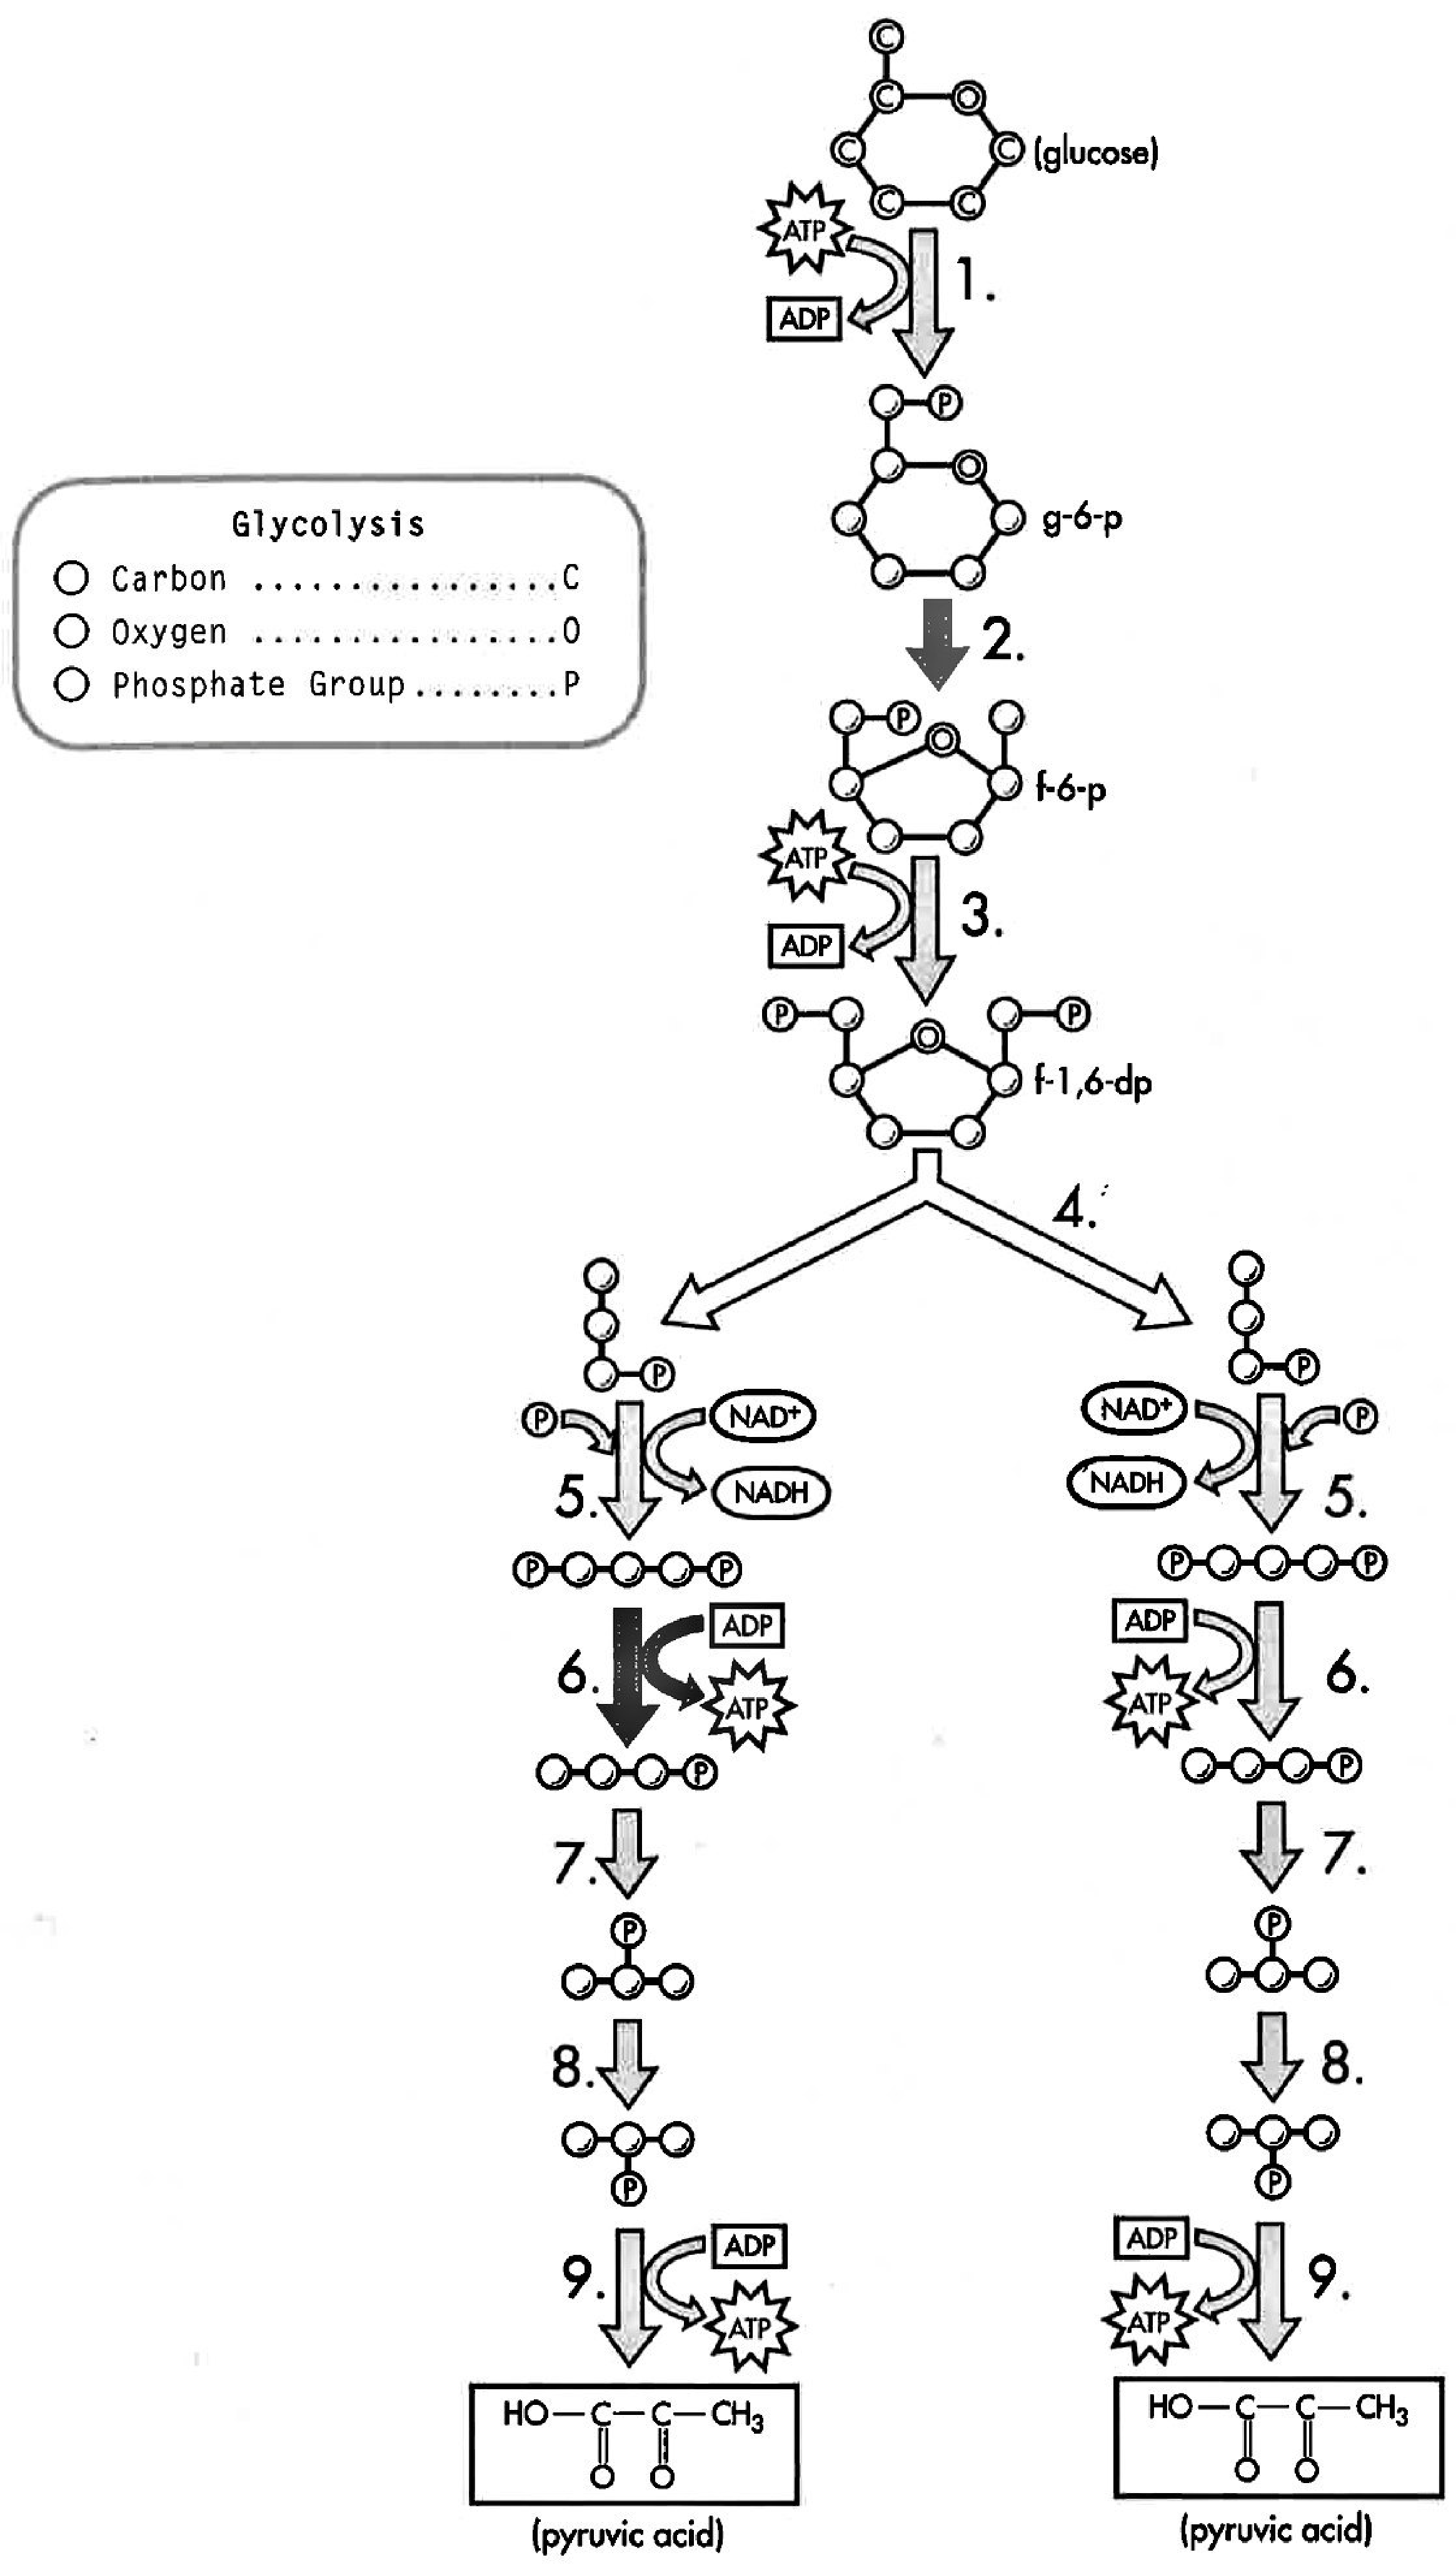
\includegraphics[width=1\linewidth]{../images/BiolColBook_039_v1.pdf}}   \captionof{figure}[Glycolysis scheme taken from Biology Coloring book, chapter 2]{Glycolysis, the break down of glucose, takes part in the cytoplasm. Colour and explain this figure!}   \label{fig:GlykolyseMarkl}
	\vspace{2pt}
	\end{minipage}
	      }{   
			\vspace{4pt}
	\begin{minipage}[htbp]{0.9\columnwidth}
	\centering {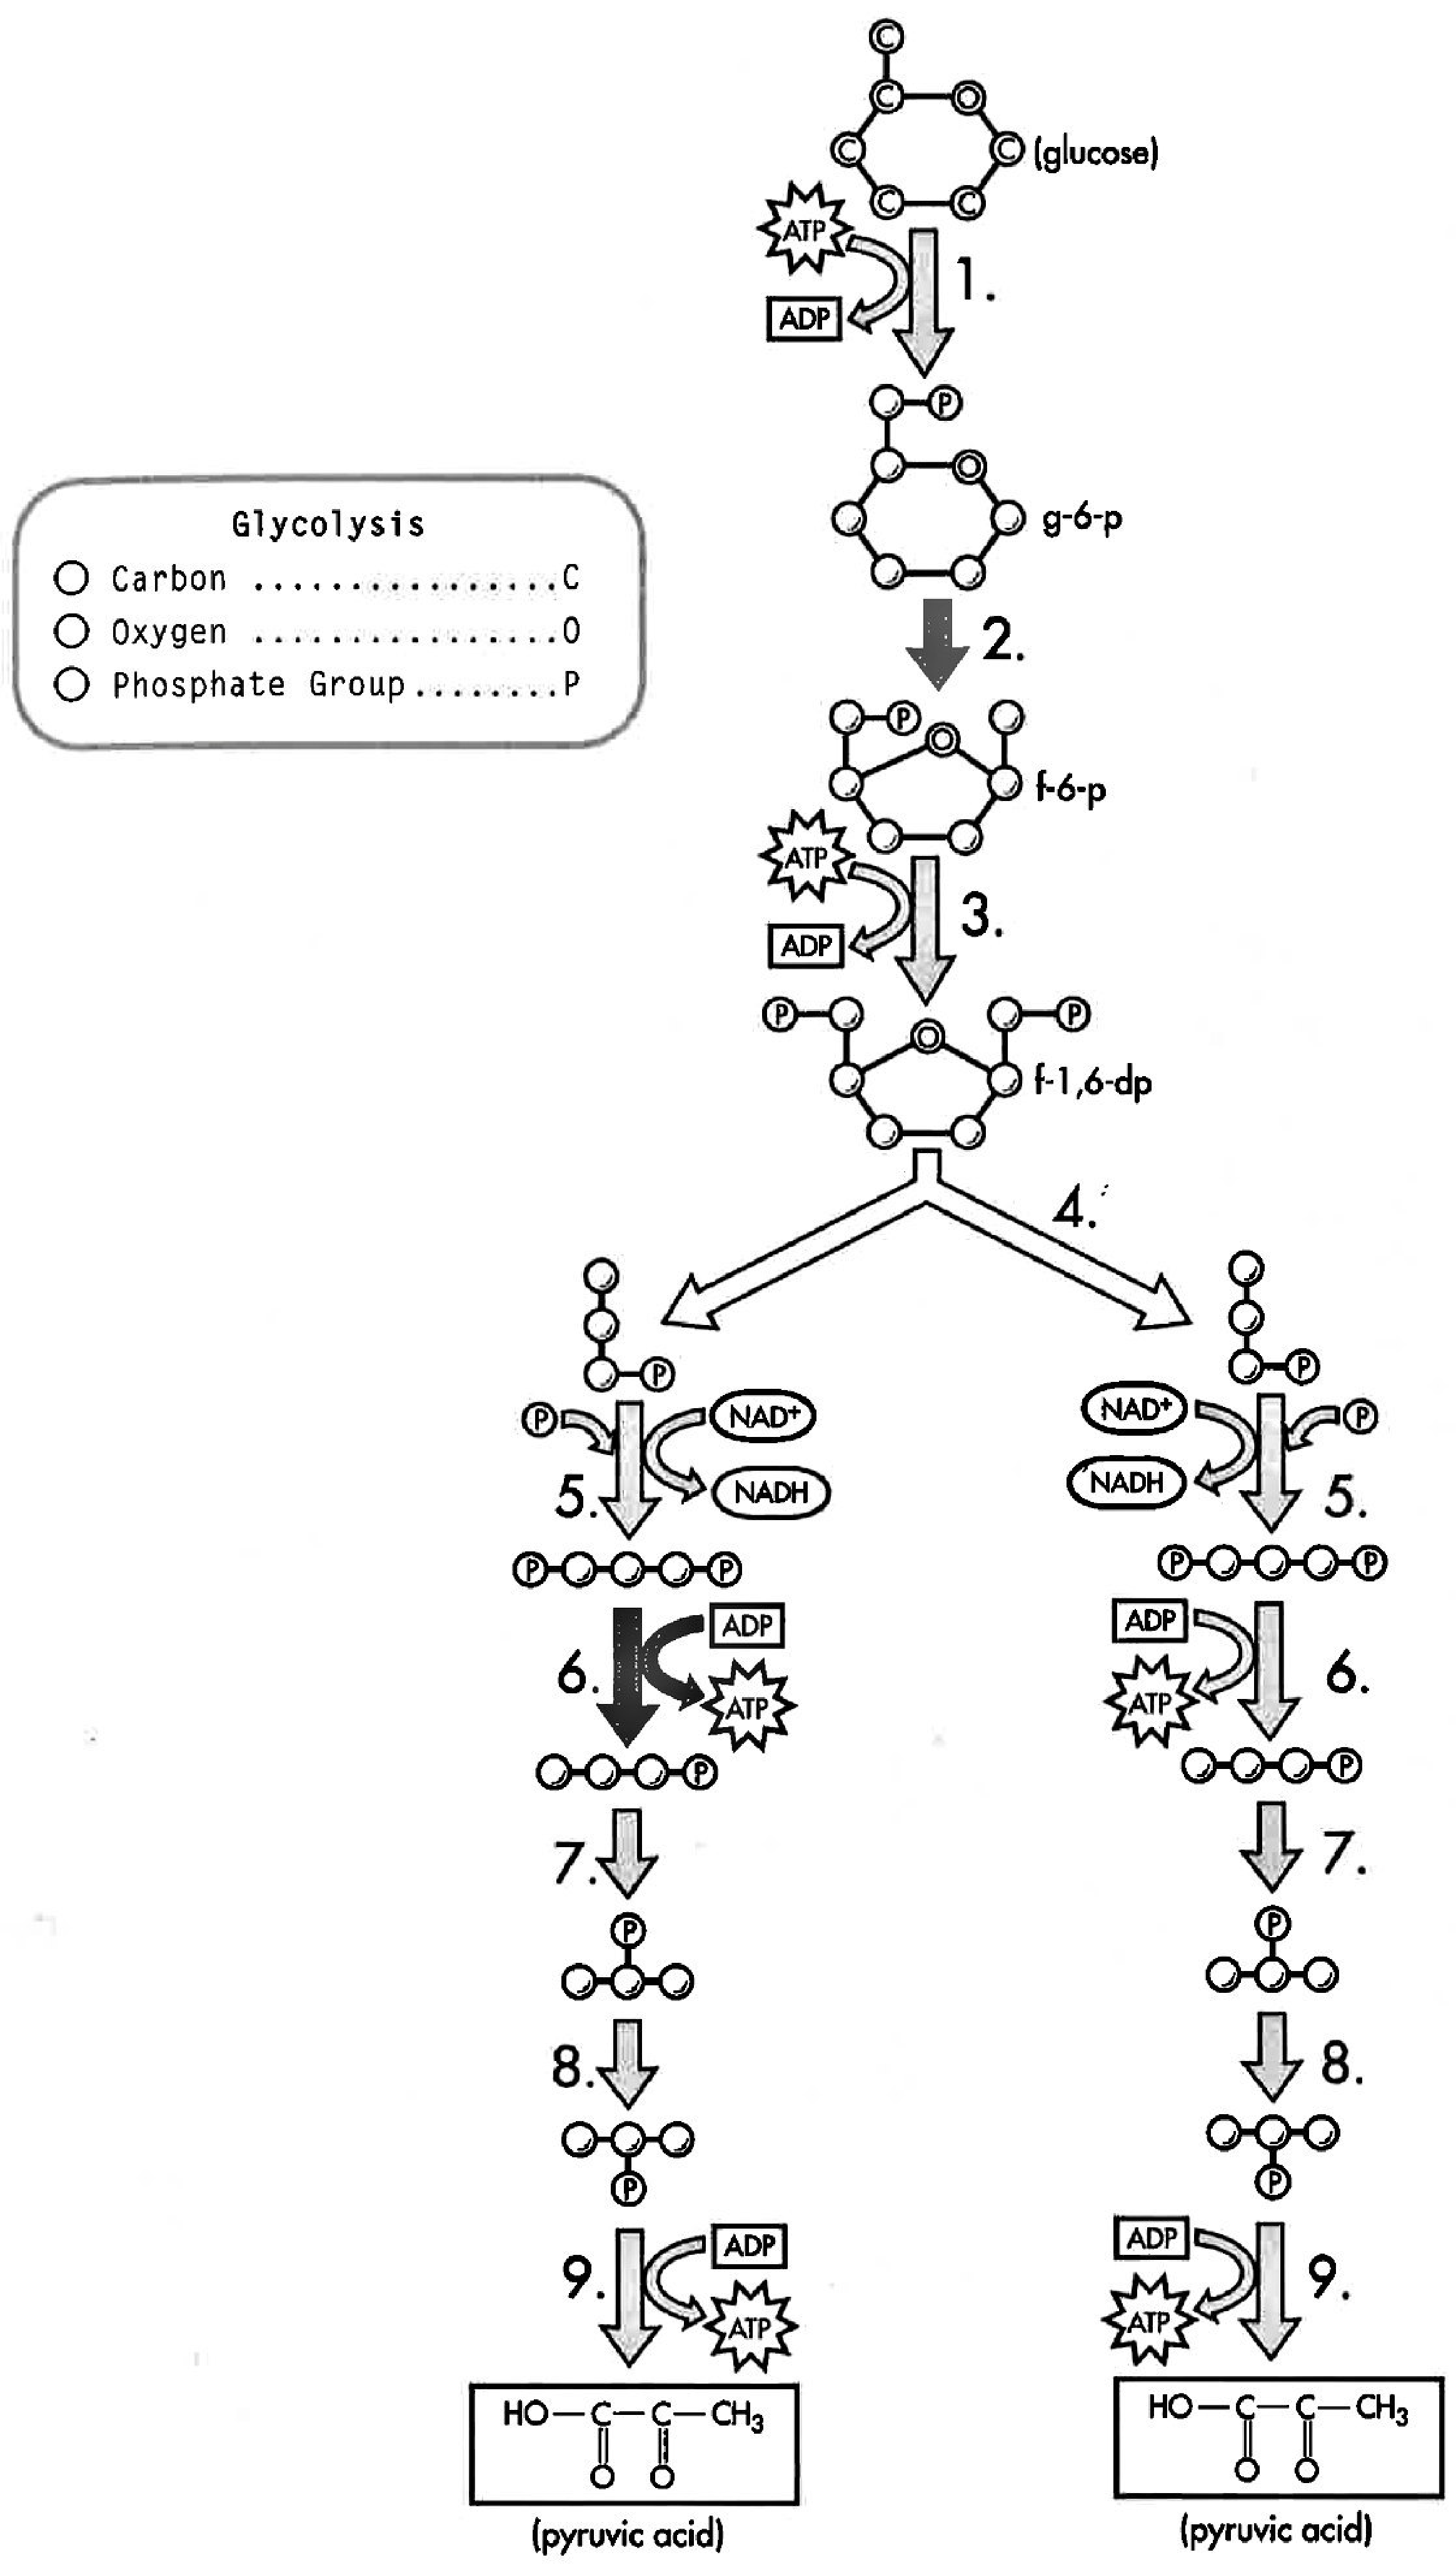
\includegraphics[width=1\linewidth]{../images/BiolColBook_039_v1.pdf}}   \captionof{figure}[Glycolysis scheme taken from Biology Coloring book, chapter 2]{Glycolysis, the break down of glucose, takes part in the cytoplasm. Colour and explain this figure!}   \label{fig:GlykolyseMarkl}
	\vspace{2pt}
	\end{minipage}
	      }	      
	      
	      \todol{get the answer figure ready!}
	      
\clearpage	        \areaset[0cm]{16cm}{27.5cm}  
\subsection{The Krebs cycle}
\marginnote{\caution[c][BrickRed][Starr!]{Read \ding{229} Starr ch 7.4}}[1cm]

\Ersatz{
		\vspace{1cm}
	\begin{minipage}[htbp]{0.95\columnwidth}
	\centering {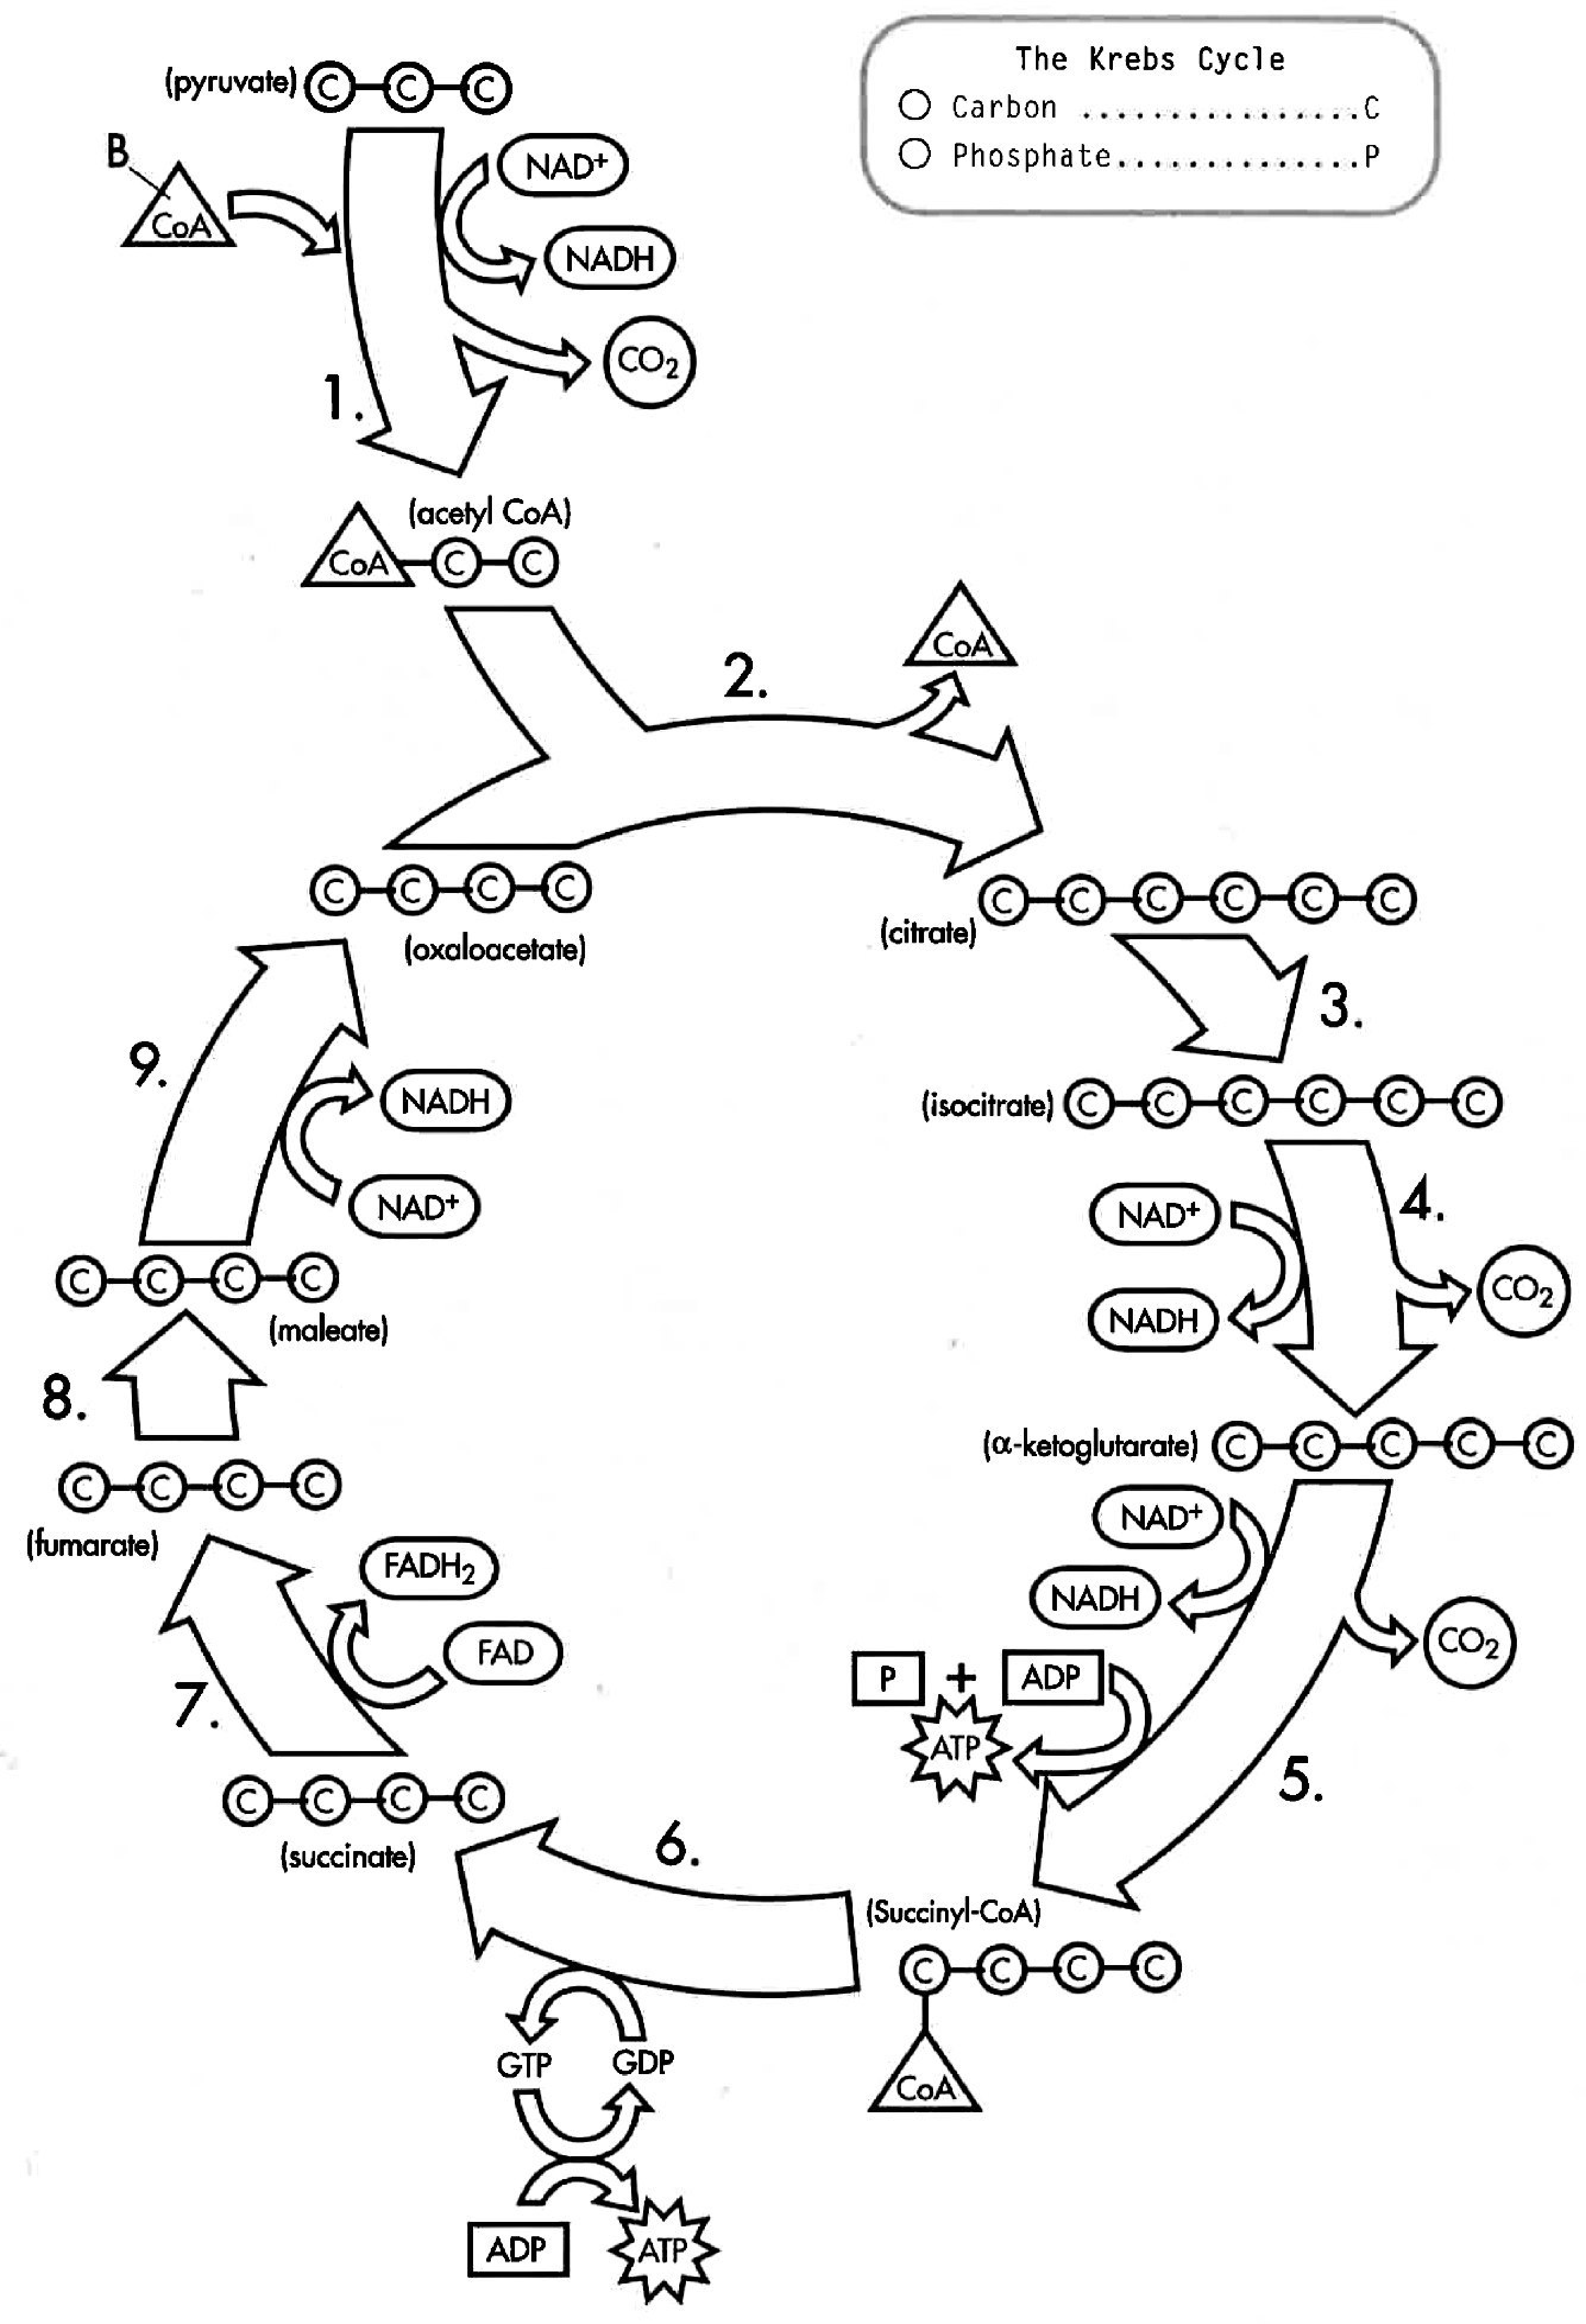
\includegraphics[width=1\linewidth]{../images/BiolColBook_041_v1.pdf}}   \captionof{figure}[Krebs cycle scheme taken from Biology Coloring book, chapter 2]{The Krebs cycle - the central piece of the metabolic system in any cell. Colour and explain this figure!}   \label{fig:KrebsCycleColourBook}
	\vspace{2pt}
	\end{minipage}
	}{
		\vspace{1cm}
	\begin{minipage}[htbp]{0.95\columnwidth}
	\centering {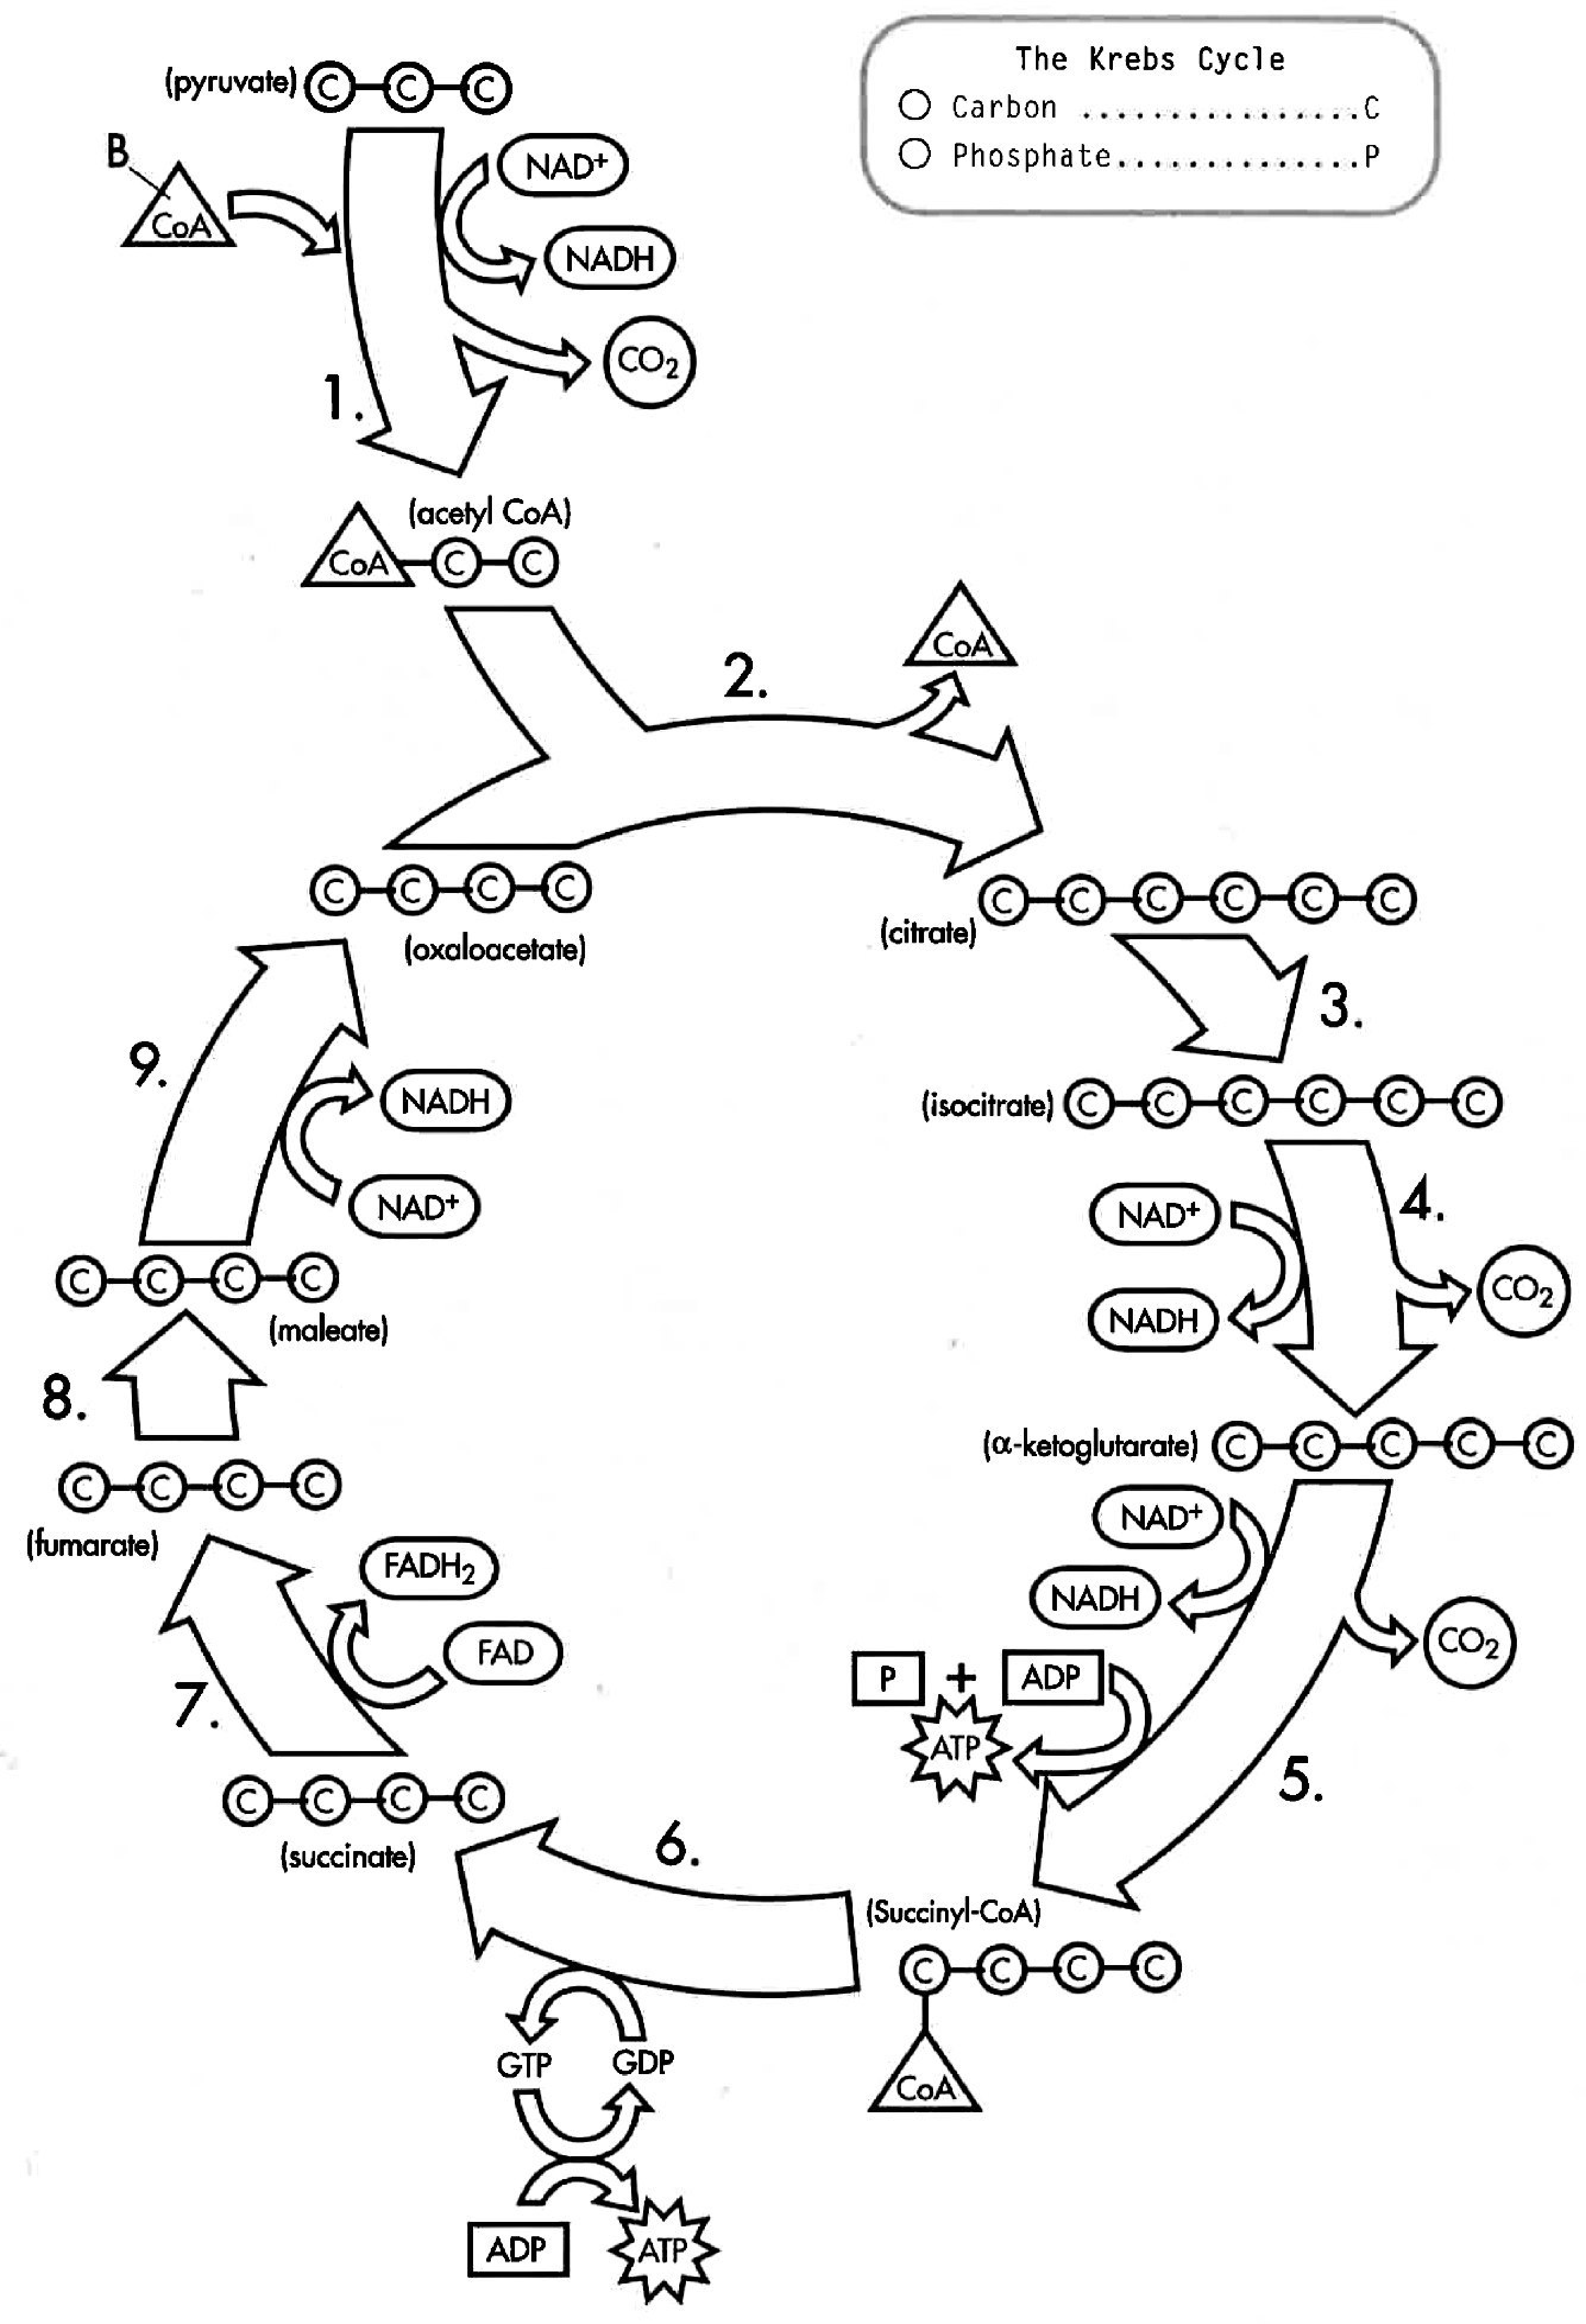
\includegraphics[width=1\linewidth]{../images/BiolColBook_041_v1.pdf}}   \captionof{figure}[Krebs cycle scheme taken from Biology Coloring book, chapter 2]{The Krebs cycle - the central piece of the metabolic system in any cell. Colour and explain this figure!}   \label{fig:KrebsCycleColourBook}
	\vspace{2pt}
	\end{minipage}
	}
	      
	      \todol{get the answer figure ready!}
	      
	      
\clearpage
\subsection{Electron Transfer Phosporylation}
\marginnote{\caution[c][BrickRed][Starr!]{Read \ding{229} Starr ch 7.5}}[0cm]
\Ersatz{
		\vspace{1.5cm}
	\begin{minipage}[htbp]{1\columnwidth}
	\centering {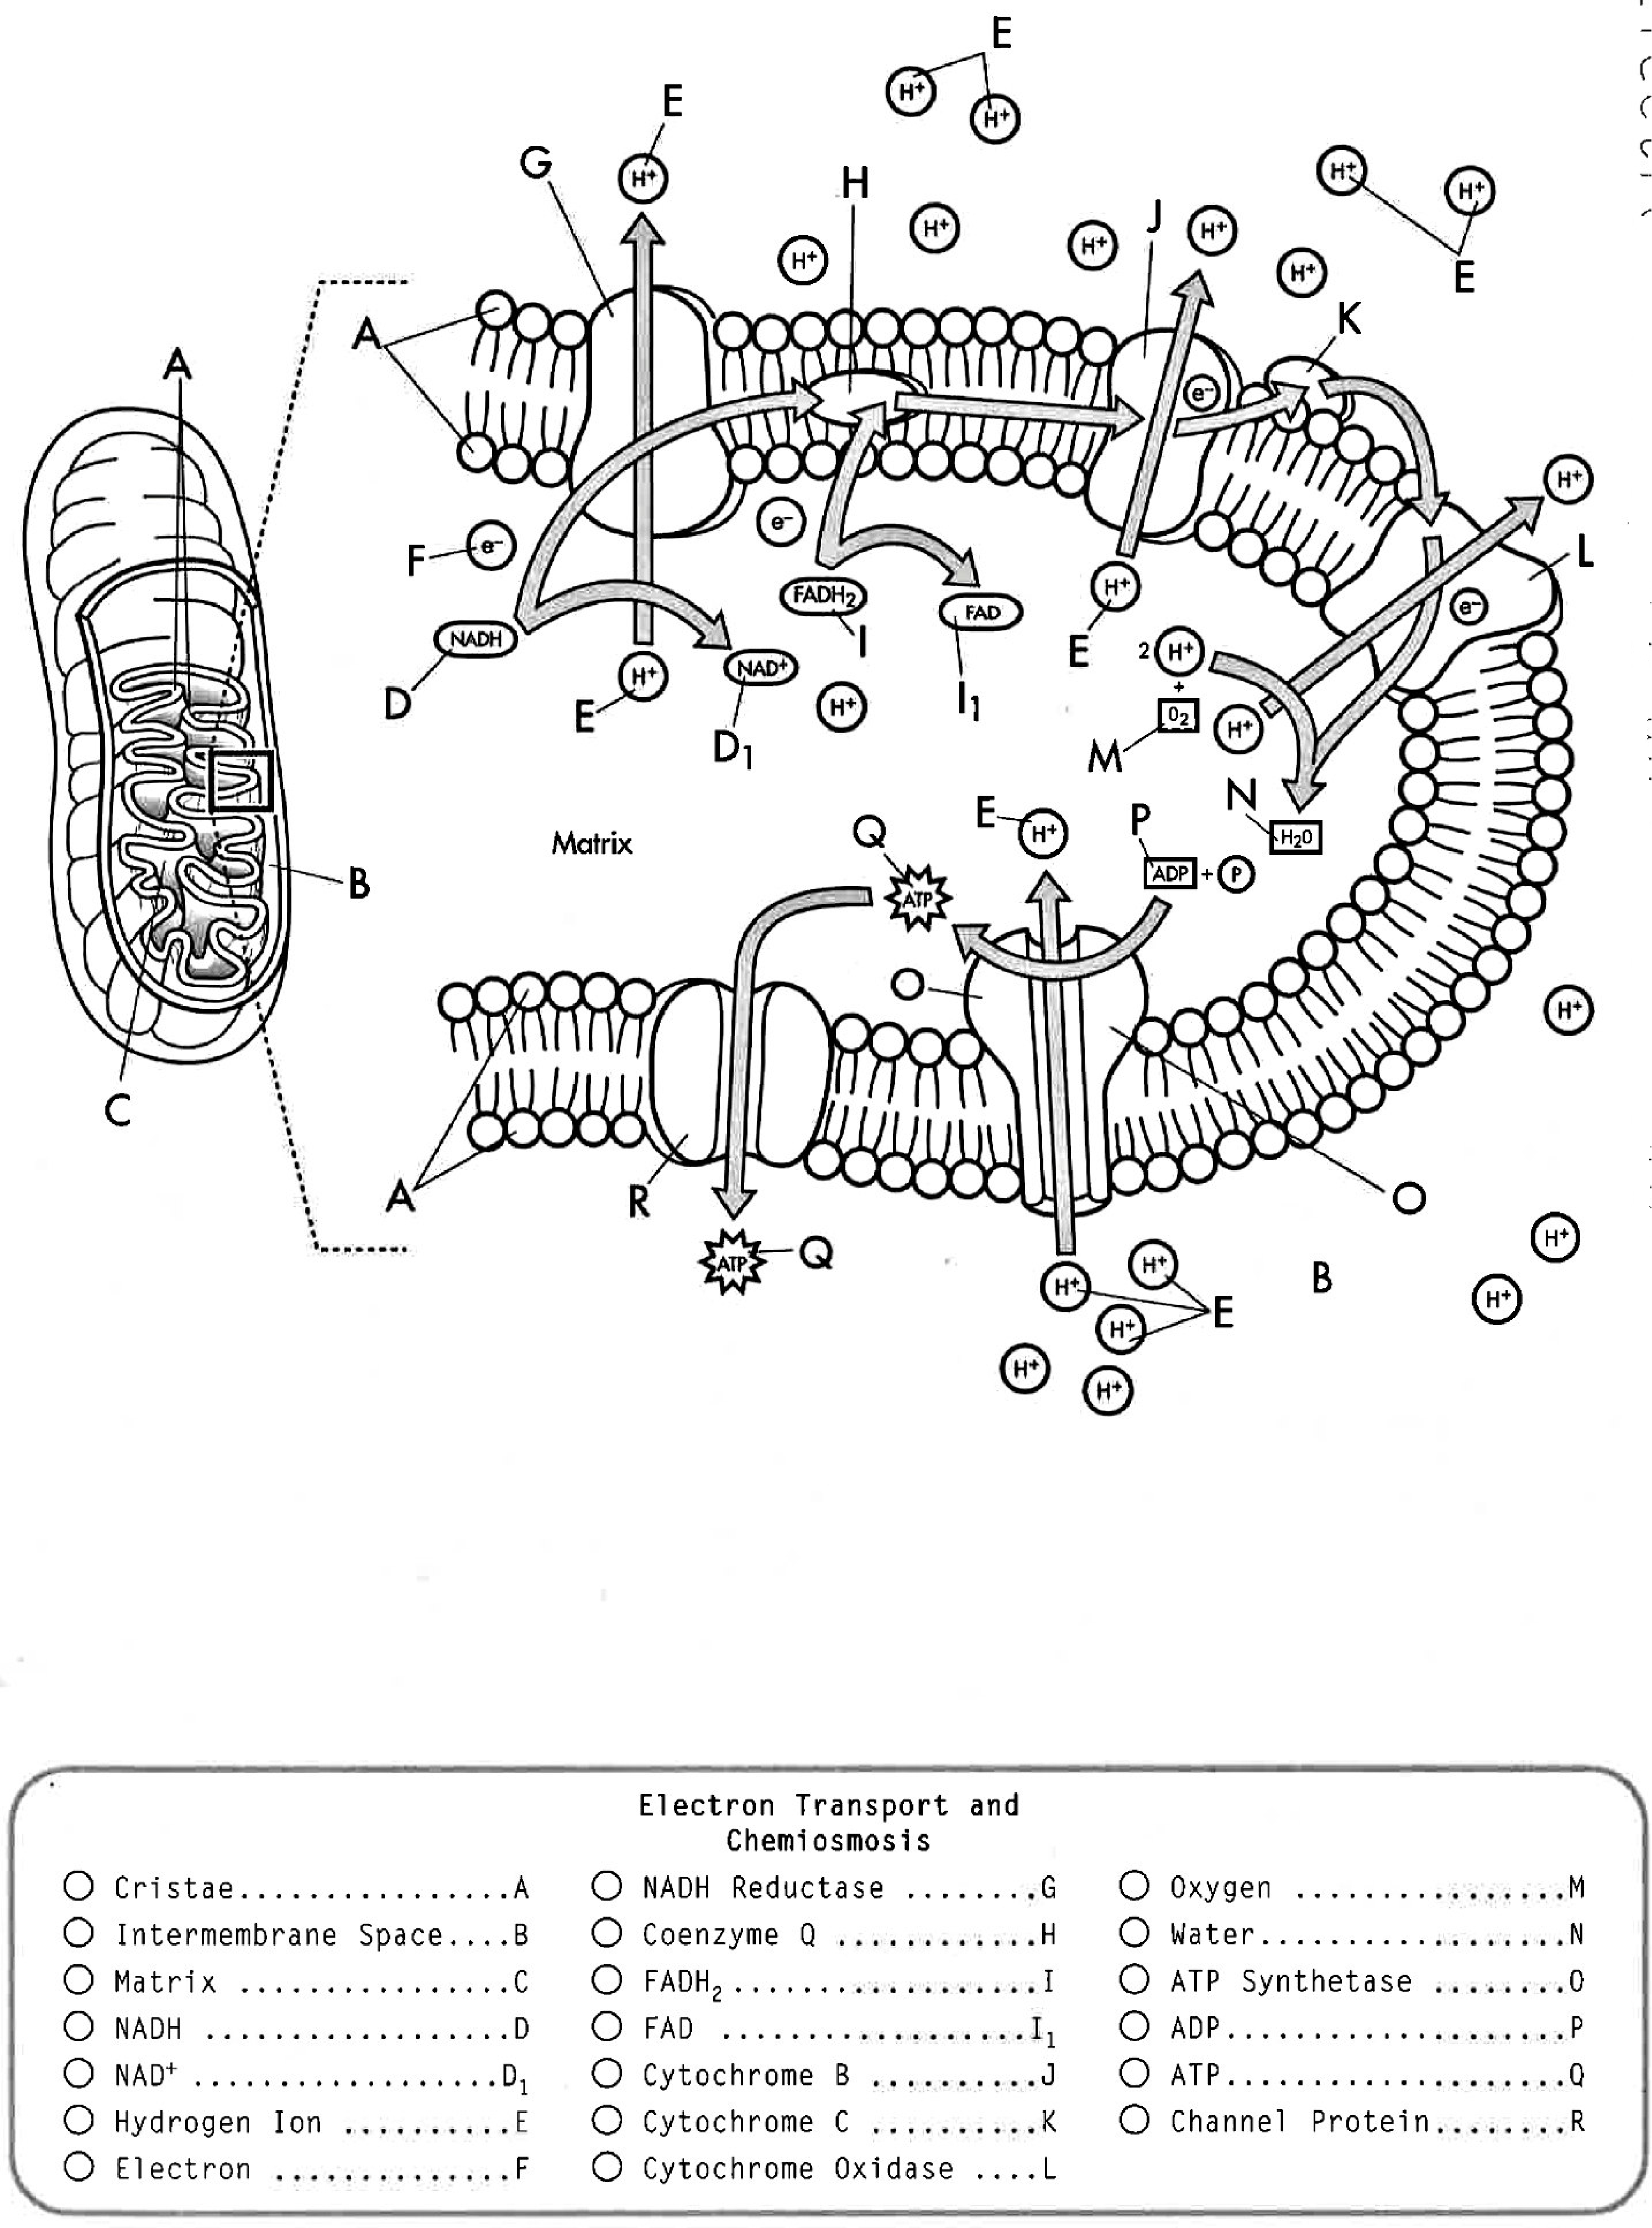
\includegraphics[width=1\linewidth]{../images/BiolColBook_043_v1.pdf}}   \captionof{figure}[Electron transfer scheme taken from Biology Coloring book, chapter 2]{The Electron Transport and Chemiosmosis - a process where osmosis meets chemistry. Colour and explain this figure!}   \label{fig:ElectronTransferColourBook}
	\vspace{2pt}
	\end{minipage}
	}{
		\vspace{1cm}
	\begin{minipage}[htbp]{1\columnwidth}
	\centering {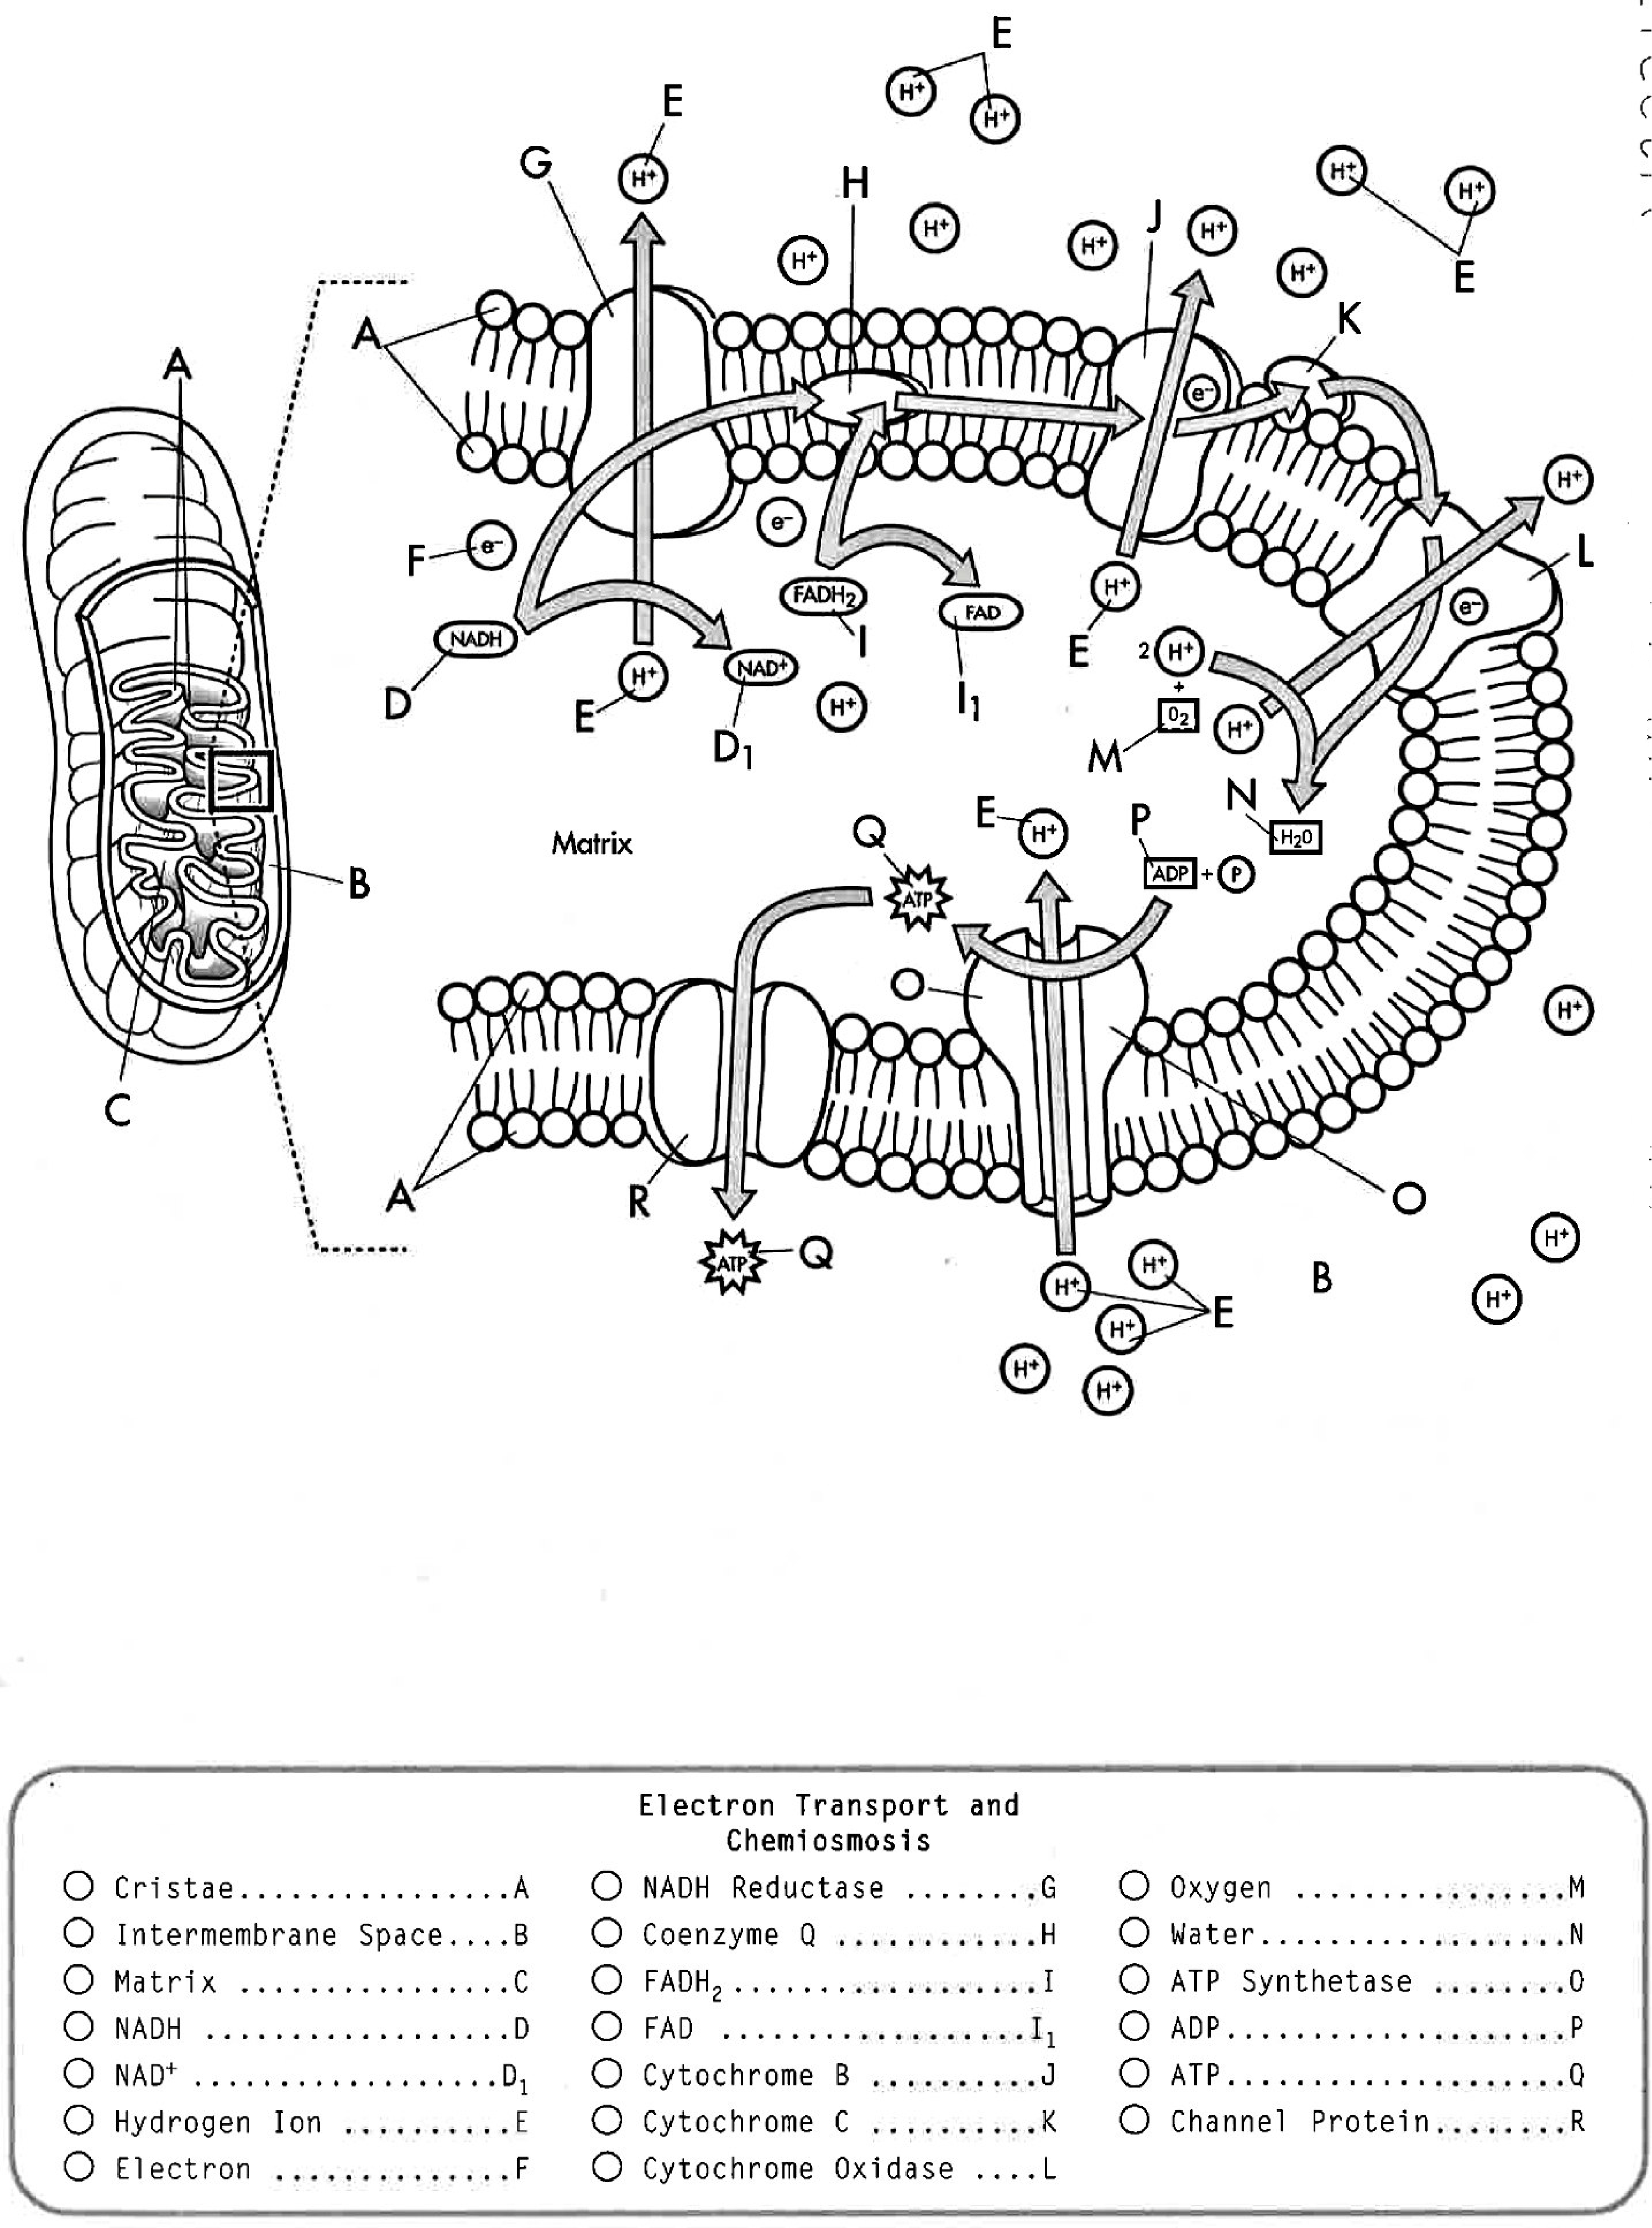
\includegraphics[width=1\linewidth]{../images/BiolColBook_043_v1.pdf}}   \captionof{figure}[Electron transfer scheme taken from Biology Coloring book, chapter 2]{The Electron Transport and Chemiosmosis - a process where osmosis meets chemistry. Colour and explain this figure!}     \label{fig:ElectronTransferColourBook}
	\vspace{2pt}
	\end{minipage}
	}



\clearpage
\subsection{Cell respiration - the overview}
	\fboxsep2pt
\begin{enumerate}[resume, leftmargin=*]
\item  Figure \ref{fig:Atmungskette} is incomplete. Label the steps (column \textit{step}), indicate the location of the steps (column \textit{place}). Add the missing items: \fbox{2  \ce{H2}}, \fbox{2  \ce{H}}, \fbox{ 2 \ce{CO2}}, \fbox{2  \ce{H2O}}, \fbox{citrate},  \fbox{succinate},  \fbox{oxalacetate},  \fbox{2 acetyl-CoA},  \fbox{2 pyruvate},  \fbox{12  \ce{H2}},  \fbox{6  \ce{O2}}, \fbox{12  \ce{H2O}}. Add the numbers of ATP generated in each step (column \textit{ATP yield}).
\end{enumerate}
\enlargethispage{2cm}

\Ersatz{
		\begin{minipage}{16cm}
			  \includegraphics[width=0.95\textwidth]{../images/CellRespirationOverview_v1.png}
		  \captionof{figure}[VERZEICHNISEINTRAG]{sum up the ATPs and  \ce{H2} molecules!} 
		  \label{fig:Atmungskette}
		\end{minipage}
		}{
				\begin{minipage}{16cm}
			  \includegraphics[width=0.95\textwidth]{../images/CellRespirationOverview_v3.png}
		  \captionof{figure}[VERZEICHNISEINTRAG]{sum up the ATPs and  \ce{H2} molecules!} 
		  \label{fig:Atmungskette}
		\end{minipage}
		}
